\section{Overview}
\subsection{Human Action Recognition}
\begin{frame}{Human Action Recognition}
    Human action recognition (HAR) can be divided into action classification and action detection.

    \begin{enumerate}
        \item<1-> Action classification is the analysis of a segmented video containing only a single action that must be classified into a defined action category (early).
              \only<1>{
                  \begin{figure}[htp]
                      \centering
                      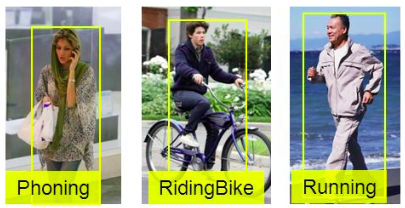
\includegraphics[width=0.6\textwidth]{topics/201010-zhang2019comprehensive/assets/img/action-classification.png}
                      \caption{Action classification}
                      \label{fig:action-classification}
                  \end{figure}
              }
        \item<2-> Action detection detects the start and end times of each action in the video, locates their position in space, and identifies the action category (more challenging).
              \only<2>{
                  \begin{figure}[htp]
                      \centering
                      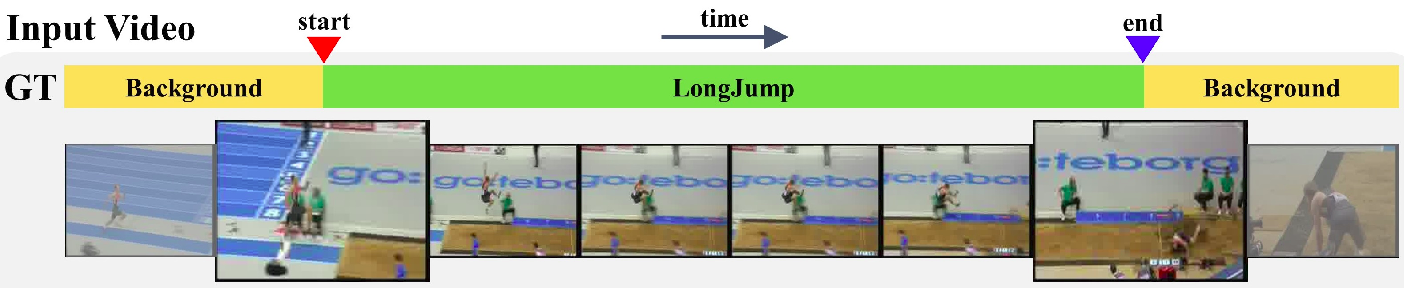
\includegraphics[width=0.8\textwidth]{topics/201010-zhang2019comprehensive/assets/img/action-detection.jpg}
                      \caption{Action detection}
                      \label{fig:action-dectection}
                  \end{figure}
              }
    \end{enumerate}


\end{frame}

\begin{frame}{Human Action Recognition}
    Techniques can be categorized into the following four classes of action semantics from low to high:
    \begin{itemize}
        \item Primitive action recognition (waving, lifting a foot, bending).
        \item Single-person action recognition (walking, punching, jumping).
        \item Interaction recognition (playing an instrument, carrying a knife).
        \item Group action recognition (parade, group meeting).
    \end{itemize}
\end{frame}

\subsection{Applications of HAR}
\begin{frame}{Applications of HAR}
    \begin{figure}[htp]
        \centering
        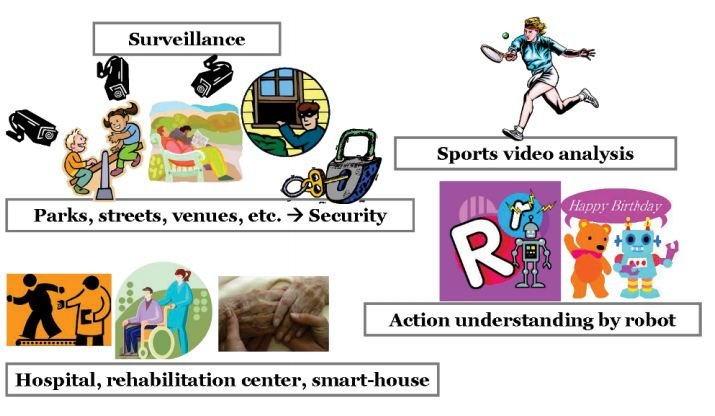
\includegraphics[width=0.7\textwidth]{topics/201010-zhang2019comprehensive/assets/img/application.png}
        \caption{Applications}
        \label{fig:applications}
    \end{figure}
\end{frame}

\subsection{Type of Dataset}
\begin{frame}{Type of Dataset}

    Most reviews of human action recognition are limited to approaches based on specific data: RGB, Skeleton, Depth \cite{shahroudy2016ntu}.

    \begin{multicols}{2}
        \begin{figure}[htp]
            \centering
            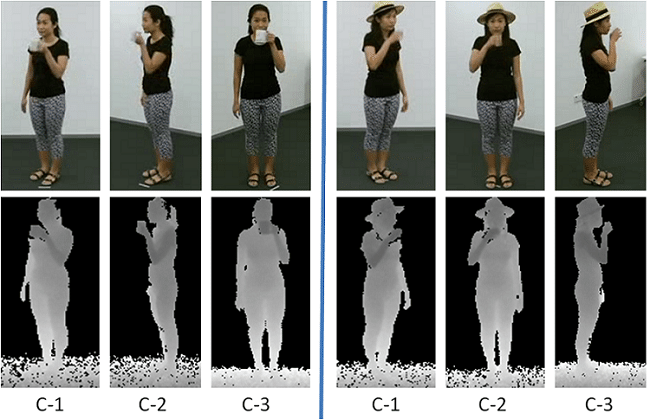
\includegraphics[height=4cm]{topics/201010-zhang2019comprehensive/assets/img/depth_data_ex.png}
            \caption{Depth data}
            \label{fig:depth_data_ex}
        \end{figure}
        \begin{figure}[htp]
            \centering
            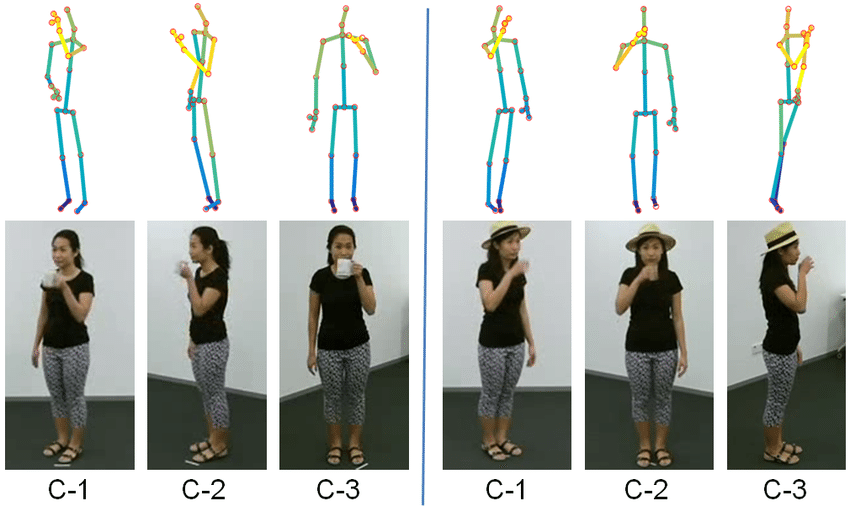
\includegraphics[height=4cm]{topics/201010-zhang2019comprehensive/assets/img/skeleton_data_ex.png}
            \caption{Skeleton data}
            \label{fig:skeleton_data_ex}
        \end{figure}
    \end{multicols}
\end{frame}